\thispagestyle{lichsutoanhocnone}
\pagestyle{lichsutoanhoc}
\graphicspath{{../lichsutoanhoc/pic2/}}
\everymath{\color{lichsutoanhoc}}
\blfootnote{$^1$\color{lichsutoanhoc}Cộng tác viên Viện Toán học.}
\begingroup
\AddToShipoutPicture*{\put(0,616){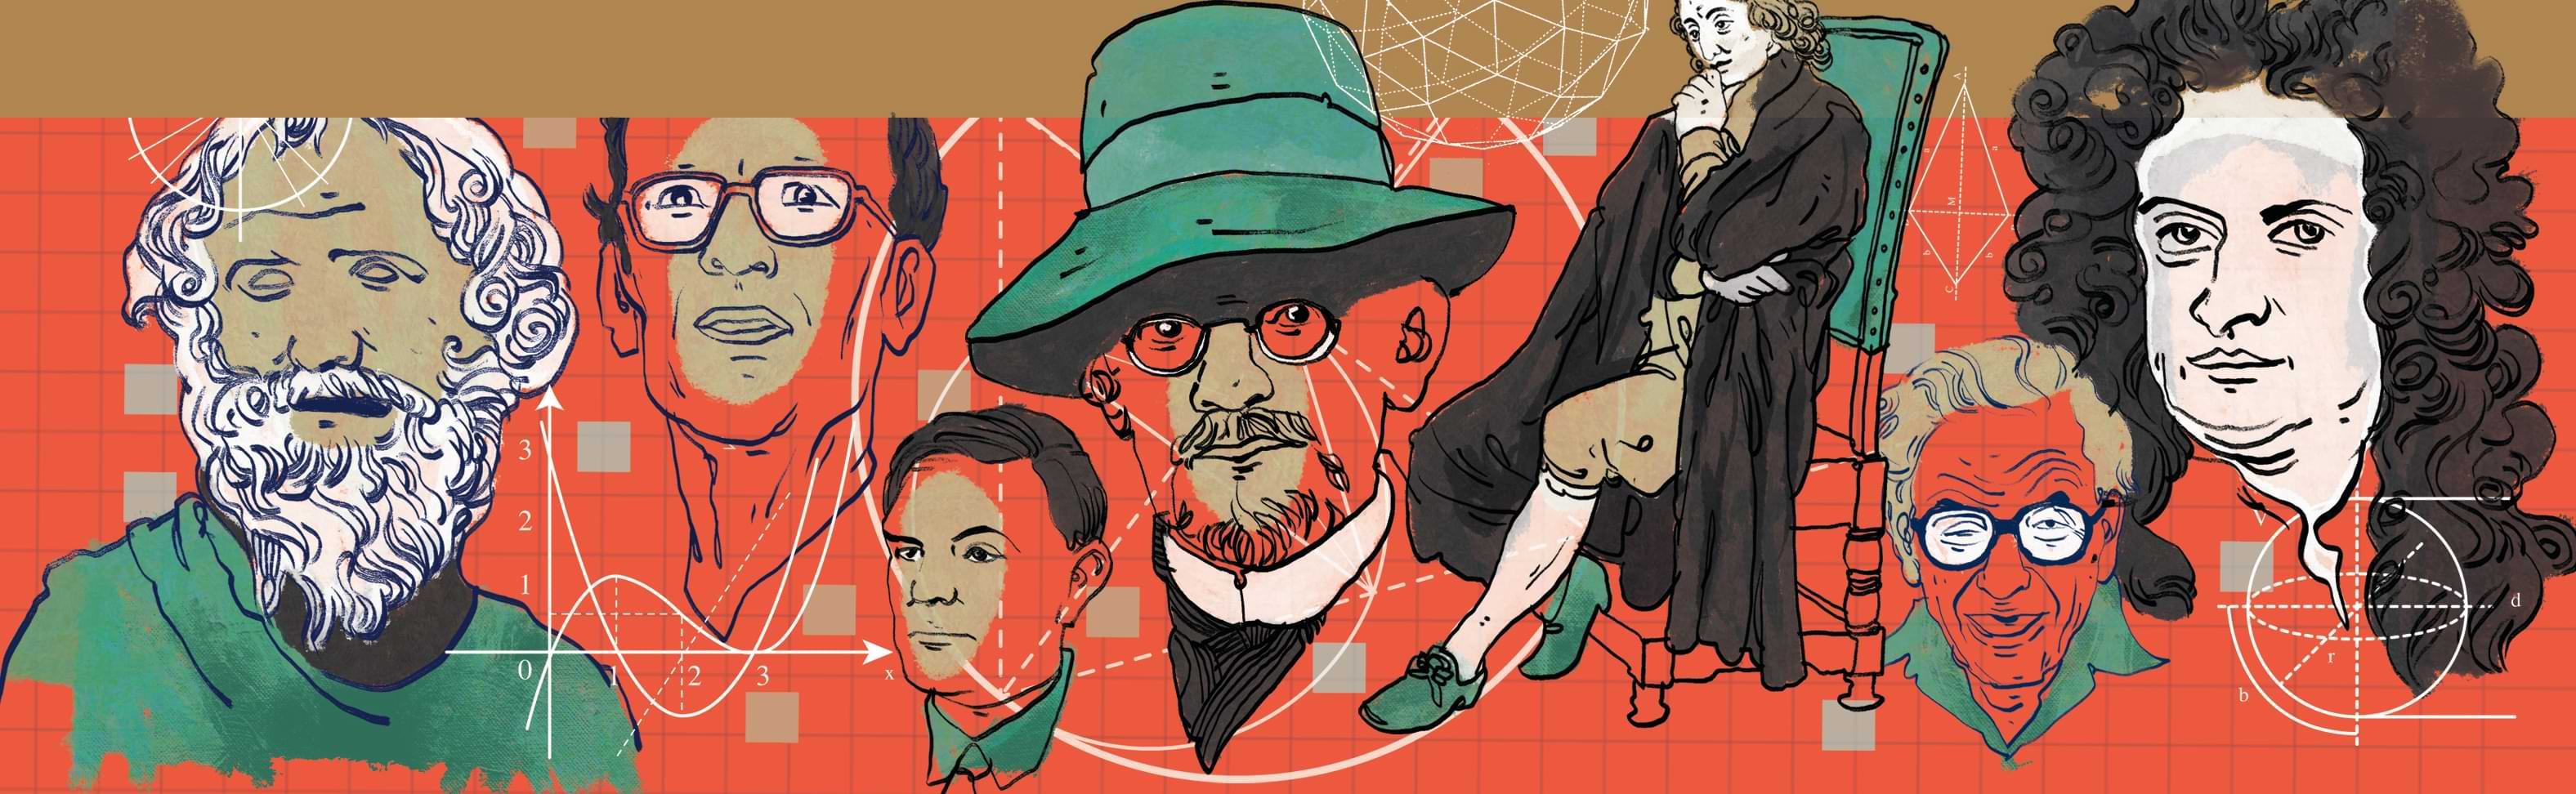
\includegraphics[width=19.3cm]{../bannerlichsu}}}
\AddToShipoutPicture*{\put(60,470){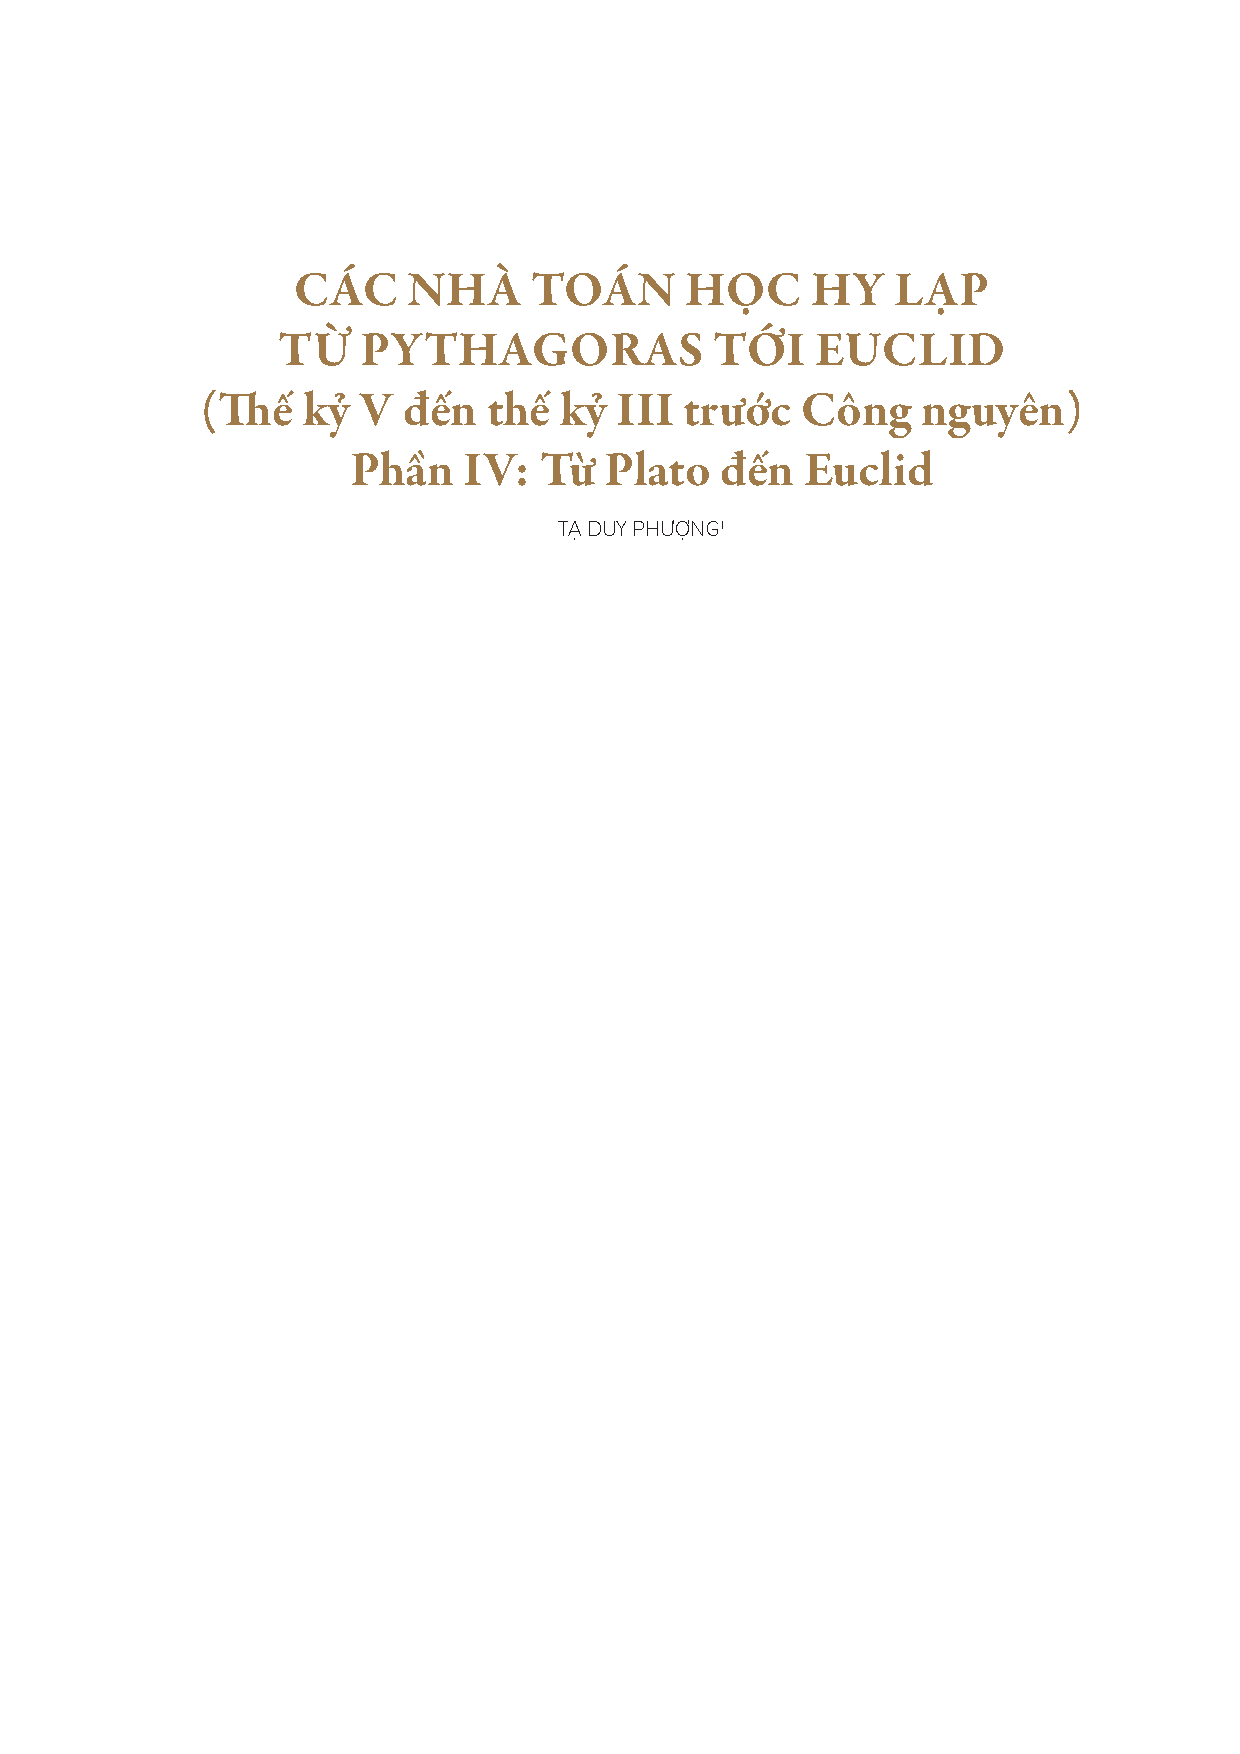
\includegraphics[scale=1]{../tieude3.pdf}}}
\centering
\endgroup

\vspace*{236pt}

\begin{multicols}{2}
	$\pmb{1}$. \textbf{\color{lichsutoanhoc}Democritus xứ Abdera} 
	\vskip 0.1cm
	Xã hội loài người đã và đang trải qua năm giai đoạn phát triển: Tiền sử (Prehistory), Cổ đại (Classical), Trung đại (Middle), Cận đại (Early Modern) và Hiện đại (Modern). \textit{Thời đại anh hùng} thuộc vào thời kỳ Cổ đại. Trong Thời đại anh hùng, đặc biệt là ở Hy Lạp và La Mã, các vị thần và á thần, các anh hùng vĩ đại trong truyền thuyết (Achilles, Hercules, Agamemnon, ...)  đã thực hiện những hành động anh hùng và tỏa sáng. 
	\vskip 0.1cm
	Thời đại anh hùng đã tạo ra nửa tá nhân vật vĩ đại trong toán học, trong số đó phải kể đến Democritus xứ Abdera (khoảng $460-370$ TCN), ngày nay được tôn vinh như một người đề xướng học thuyết duy vật nguyên tử, nhưng đương thời ông cũng được tôn vinh như một nhà hình học. Ông được cho là đã đi du lịch nhiều hơn bất kỳ ai trong thời của mình -- ông đã đến Athens, Ai Cập, Lưỡng Hà và có thể cả Ấn Độ -- tiếp thu những gì học được, và những thành tựu của riêng ông trong toán học là xuất sắc. Ông đã viết một số công trình toán học, nhưng ngày nay không còn tồn tại. 
	\vskip 0.1cm
	Chìa khóa cho toán học của Democritus được tìm thấy trong học thuyết vật lý về nguyên tử. Ông lập luận, về mức độ nhỏ vô hạn và đa dạng vô hạn (về kích thước và hình dạng), các nguyên tử di chuyển không ngừng trong không gian trống.
	\vskip 0.1cm 
	Thuyết vật lý nguyên tử của Democritus có thể đã xuất phát từ thuyết nguyên tử hình học của Pythagoras, và không có gì ngạc nhiên khi các vấn đề toán học mà Democritus quan tâm chủ yếu là những thứ đòi hỏi cách tiếp cận đại lượng vô cùng bé. Ví dụ, người Ai Cập nhận thức được rằng thể tích của một kim tự tháp bằng một phần ba tích của đáy và chiều cao, nhưng chứng minh điều này gần như chắc chắn nằm ngoài khả năng của họ, vì nó đòi hỏi các kiến thức giải tích.  Archimedes đã viết rằng kết quả này là của Democritus.  Archimedes cũng gán cho Democritus định lý nói  rằng thể tích của một hình nón bằng một phần ba thể tích của hình trụ tròn ngoại tiếp. Kết quả này có lẽ đã được Democritus coi là hệ quả của định lý về kim tự tháp, vì hình nón về cơ bản là một hình chóp có đáy là một đa giác đều có vô số cạnh.
	\vskip 0.1cm
	Lý thuyết nguyên tử hình học của Democritus ngay lập tức đối đầu với nhiều vấn đề. Ví dụ: Nếu các phần liền kề có diện tích bằng nhau, thì vì tất cả các phần đều bằng nhau, tổng sẽ là một lăng trụ hoặc một hình trụ và không phải là một hình chóp hoặc một hình nón. 
	\vskip 0.1cm
	Mặt khác, nếu các phần liền kề không bằng nhau, tổng sẽ là một kim tự tháp có bậc hoặc một hình nón có bậc chứ không phải là hình có bề mặt nhẵn. Vấn đề này không giống như những khó khăn với số vô tỷ và với những nghịch lý của chuyển động.
	\vskip 0.1cm
	Có lẽ, trong tác phẩm \textit{On the Irrational} (Về Vô tỷ), Democritus đã phân tích những khó khăn gặp phải, nhưng không có cách nào để biết những nỗ lực của ông có thể đã đi theo hướng nào.
	\vskip 0.1cm
	Democritus không được ưa chuộng trong hai trường phái triết học thống trị thế kỷ tiếp theo, của Plato và Aristotle, có thể họ đã khuyến khích việc coi thường các ý tưởng của Democritus. 
	\vskip 0.1cm
	Di sản toán học chính của Thời đại anh hùng có thể được tóm gọn trong sáu vấn đề: cầu phương hình tròn, nhân đôi thể tích hình lập phương, chia ba một góc, tỷ lệ giữa các đại lượng không thông ước, các nghịch lý về chuyển động, và phương pháp vô cùng bé. 
	\vskip 0.1cm
	Những bài toán này liên quan, ở mức độ nào đó, với những người cùng thời: Hippocrates, Archytas, Hippias, Hippasus, Zeno và Democritus. 
	\vskip 0.1cm
	Thời đại nào cũng có những tài năng, nhưng có lẽ không có thời đại nào có thể thực hiện một cuộc tấn công táo bạo vào rất nhiều các vấn đề toán học với nguồn tài nguyên phương pháp luận không đầy đủ như vậy. Vì lý do này mà thời kỳ từ Anaxagoras đến Archytas được gọi là ``Thời đại anh hùng" trong toán học.
	\vskip 0.1cm
	$\pmb{2.}$ \textbf{\color{lichsutoanhoc}Eudoxus}
	\vskip 0.1cm
	 Nhà toán học Hy Lạp lỗi lạc nhất trước Archimedes có lẽ là Eudoxus xứ Cnidos ($408 - 355$ TCN).
	 \vskip 0.1cm
	Ra đời khoảng năm $408$ TCN ở Cnidos trên Biển Đen, ở tuổi $23$, Eudoxus bắt đầu học hình học với Archytas xứ Tarentum, và học triết học và hùng biện với Plato ở Athens. Eudoxus, quá nghèo để sống ở Athens, đã ở trọ với giá rẻ mạt tại thị trấn bến cảng Piraeus, mỗi ngày ông phải đi bộ hai dặm ($1$ dặm = $1{,}6$ km) đến Học viện Plato. Sau đó, ông đến Ai Cập, nơi ông ở lại trong $16$ tháng. Ông kiếm sống bằng nghề dạy học, thành lập một trường học tại Cyzicus ở Tây Bắc Tiểu Á, trường đã thu hút rất nhiều học sinh. Vào năm $365$ TCN, Eudoxus trở lại Athens cùng với một số lượng lớn các học trò. Ở đó, ông trở thành một đồng nghiệp của Plato.
	Eudoxus cũng đã mở một trường học ở Athens, có một thời gian là đối thủ cạnh tranh của Học viện Plato.
	\vskip 0.1cm
	Eudoxus là nhà toán học và thiên văn học hàng đầu của thời đại mình. Eudoxus đã giải quyết những khủng hoảng của toán học thời đại ông. Ông có ba cống hiến cho toán học: lý thuyết tổng quát về tỷ lệ, bổ sung nhiều kết quả nghiên cứu về tỷ lệ vàng, và phát minh ra một quy trình được gọi là \textit{phương pháp vét kiệt}.
	\vskip 0.1cm 
	\textit{\color{lichsutoanhoc}Lý thuyết tổng quát về tỷ lệ} 
	\vskip 0.1cm
	Việc khám phá ra số vô tỷ đã gây ra một sự khủng hoảng trong toán học, vì nó đã làm lung lay niềm tin về số (hữu tỷ) là bản chất của mọi thứ và làm lý thuyết về tỷ lệ của người Pythagoras không còn vững vàng. Hai đại lượng, chẳng hạn như đường chéo và cạnh của hình vuông, không thông ước, vì độ dài của chúng không có tỷ lệ là một số (hữu tỷ). Vậy thì làm thế nào để so sánh các tỷ lệ của các đại lượng vô ước?
	\vskip 0.1cm
	Người Pythagoras đã sử dụng ý tưởng rằng bốn đại lượng theo tỷ lệ, $a:b = c : d$,  nếu hai tỷ lệ $a:b$  và $c:d$ có cùng một cách trừ. Nghĩa là, số nhỏ hơn trong mỗi tỷ lệ có thể được bớt đi ở số lớn hơn cùng một số lần và phần dư trong mỗi trường hợp có thể được bớt đi cùng một số lần ở số nhỏ hơn, và phần dư mới lại có thể được bớt đi cùng một số lần ở phần dư đầu tiên, v.v. 
	\vskip 0.1cm
	Định nghĩa như vậy rất khó sử dụng (khi áp dụng cho số vô tỷ), do đó lý thuyết mới về tỷ lệ là một thành tựu rực rỡ của Eudoxus và nó đã được đưa vào Quyển V của \textit{Cơ sở} của Euclid.
	\vskip 0.1cm
	Một tuyên bố quan trọng của Euclid là các đại lượng được cho có một tỷ lệ với nhau nếu bội số của một trong hai số có thể vượt quá số kia. 
	\vskip 0.1cm
	Đây thực chất là tiên đề Archimedes -- mà Archimedes gán cho Eudoxus. Khái niệm tỷ lệ của Eudoxus do đó loại trừ số không và làm rõ nghĩa độ lớn cùng loại là gì. Ví dụ: một đoạn thẳng không được so sánh theo tỷ lệ với diện tích; cũng như diện tích không được so sánh với thể tích.
	\vskip 0.1cm
	Sau những nhận xét sơ bộ về tỷ lệ, Euclid đưa ra Định nghĩa $5$ trong Quyển V của \textit{Cơ sở} về phát biểu nổi tiếng của Eudoxus: \textit{Các độ lớn được cho là theo cùng một tỷ lệ, cái thứ nhất so với cái thứ hai và cái thứ ba so với cái thứ tư, khi nếu lấy các bội của cái thứ nhất và cái thứ ba với cùng một số bất kỳ, và các bội của cái thứ hai và cái thứ tư với cùng một số bất kỳ, hai bội đầu sẽ cùng lớn hơn, cùng bằng hoặc cùng bé hơn hai bội sau một cách tương ứng} ([$1$], trang $80$, xem thêm [$2$], trang $236$).
	\vskip 0.1cm
	Nghĩa là, $\dfrac{a}{b} = \dfrac{c}{d}$  nếu và chỉ nếu với các số nguyên dương bất kỳ $m$  và $n$,  nếu $ma < nb$,  thì $mc < nd$,  hoặc nếu $ma = nb$,  thì $mc = nd$,  hoặc nếu $ma > nb$  thì $mc > nd$. 
	\vskip 0.1cm
	Định nghĩa của Eudoxus về sự bằng nhau của tỷ lệ không khác gì phép nhân chéo được sử dụng ngày nay cho phân số $\dfrac{a}{b} = \dfrac{c}{d}$ nếu $ad = bc$ -- một sự tương đương với việc đưa về mẫu số chung.  Ví dụ, để chứng tỏ rằng $\dfrac{3}{6}$  bằng $\dfrac{4}{8}$  ta nhân $3$ và $6$ với $4$, được $12$ và $24$, và nhân $4$ và $8$ với $3$, thu được cùng một cặp số $12$ và $24$\footnote[2]{\color{lichsutoanhoc}Ở đây chúng ta đã đổi vai trò của ``cái thứ hai" và ``cái thứ ba" trong định nghĩa của Eudoxus -- Pi.}.
	\vskip 0.1cm 
	Cần lưu ý rằng, định nghĩa này không xa mấy so với định nghĩa về số thực ở thế kỷ $19$ bởi lát cắt Dedekind, vì nó phân lớp số hữu tỷ  $\dfrac{m}{n}$  thành hai lớp, theo $ma \le nb$  và $ma > nb$.
	\vskip 0.1cm 
	Vì có vô số số hữu tỷ, người Hy Lạp đã phải đối mặt với khái niệm mà họ muốn tránh -- đó là tập hợp vô hạn -- nhưng ít nhất dựa trên khái niệm về tỷ lệ của Eudoxus, họ đã có thể đưa ra các chứng minh thỏa đáng cho các định lý liên quan đến tỷ lệ.
	\vskip 0.1cm
	\textit{\color{lichsutoanhoc}Phương pháp vét kiệt}
	\vskip 0.1cm
	Cuộc khủng hoảng về vô ước đã được giải quyết thành công, nhờ vào định nghĩa của Eudoxus về tỷ lệ, nhưng vẫn còn một vấn đề chưa được giải quyết -- so sánh cấu hình đường cong và đường thẳng. 
	\vskip 0.1cm
	Ở đây, có vẻ như Eudoxus đã cung cấp chìa khóa.
	\vskip 0.1cm
	Các nhà toán học trước đây dường như đã có ý mô tả các hình đa giác nội tiếp và ngoại tiếp các hình cong và tiếp tục tăng vô hạn số cạnh, nhưng họ đã không biết cách lập luận, vì khái niệm giới hạn là chưa rõ ràng vào thời điểm ấy. 
	\vskip 0.1cm
	Theo Archimedes, chính Eudoxus là người đã cung cấp bổ đề hiện mang tên Archimedes -- đôi khi được gọi là tiên đề về tính liên tục -- được dùng làm cơ sở cho phương pháp vét kiệt, tương đương  Hy Lạp của phép tính tích phân.
	\vskip 0.1cm
	Bổ đề (hoặc tiên đề) Eudoxus nói rằng hai đại lượng có một tỷ số (nghĩa là, không bằng $0$) nếu có thể tìm thấy một nhân tử để đại lượng này sẽ vượt quá đại lượng kia. Có thể phát biểu điều này trên ngôn ngữ hiện đại như sau: Cho $M > \epsilon$  và một số $0 < r < 1$. Khi ấy tồn tại số $n \in \mathbb{N}$  sao cho $M(1-r)^n < \epsilon$, tức là $\mathop {\lim }\limits_{n \to \infty } M{\left( {1 - r} \right)^n} = 0$. 
	\vskip 0.1cm
	Khẳng định này đã loại trừ lập luận mơ hồ về các đoạn thẳng không thể phân chia hoặc các số nhỏ cố định, đôi khi duy trì trong tư tưởng Hy Lạp. 
	\vskip 0.1cm
	Phương pháp vét kiệt được đề xuất bởi Eudoxus sau đó đã được Archimedes phát triển thành một công cụ mạnh mẽ để xác định diện tích hình phẳng, diện tích bề mặt và thể tích đường cong --  một tiền thân quan trọng của phép toán tích phân.
	\begin{figure}[H]
		\vspace*{-5pt}
		\centering
		\captionsetup{labelformat= empty, justification=centering}
		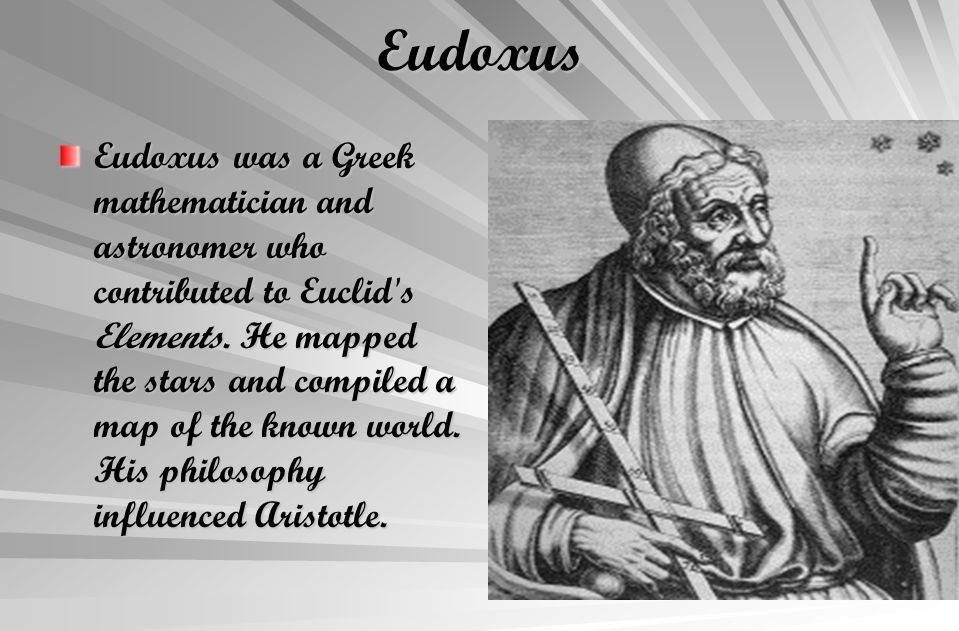
\includegraphics[width= 1\linewidth]{1}
		\vspace*{-15pt}
	\end{figure}
	\textit{\color{lichsutoanhoc}Thiên văn của Eudoxus} 
	\vskip 0.1cm
	Eudoxus không chỉ là một nhà toán học. Ông còn được biết đến như là cha đẻ của khoa học thiên văn. Plato được cho là đã cố gắng đưa ra một biểu diễn hình học về chuyển động của Mặt Trời, Mặt Trăng và năm hành tinh đã biết. Rõ ràng là người ta ngầm cho rằng các chuyển động là hợp nhất của các chuyển động tròn đều. Mặc dù có những hạn chế như vậy, Eudoxus đã có thể cung cấp cho mỗi thiên thể trong số bảy thiên thể một biểu diễn thỏa đáng thông qua một tổ hợp các quả cầu đồng tâm với tâm là Trái Đất và với các bán kính khác nhau, mỗi quả cầu quay đều quanh một trục cố định đối với bề mặt của hình cầu lớn hơn tiếp theo. Với mỗi hành tinh thì Eudoxus đưa ra một hệ thống mà những người kế vị của ông biết đến là ``Hình cầu đồng tâm". Những sơ đồ hình học này, được kết hợp bởi Aristotle vào vũ trụ học, đã thống trị tư tưởng trong gần $2000$ năm.
	\vskip 0.1cm
	Eudoxus, không nghi ngờ gì, là nhà toán học có năng lực nhất Thời kỳ Hy Lạp hóa (Hellenic period, khoảng $507 - 323$ trước Công nguyên), nhưng tất cả các tác phẩm của ông đã bị thất lạc. Trong thiên văn học, bằng sự kết hợp của các chuyển động tròn, Eudoxus đã có thể mô tả chuyển động của các hành tinh trong các quỹ đạo lặp lại dọc theo một đường cong được gọi là đường {\em hippopede}, hoặc vòng kiềng ngựa. Đường cong này, giống như một hình số tám trên một hình cầu, là một trong số ít các đường cong mới mà người Hy Lạp đã tìm ra. Vào thời điểm đó, chỉ có hai phương tiện xác định các đường cong: ($1$) thông qua sự kết hợp của các chuyển động đều và ($2$) như các giao điểm của các bề mặt hình học quen thuộc. 
	\vskip 0.1cm
	Proclus, khoảng $800$ năm sau Eudoxus, nói rằng Eudoxus đã thêm nhiều định lý tổng quát trong hình học và đã áp dụng phương pháp phân tích của Plato để nghiên cứu tỷ lệ vàng, nhưng cống hiến lớn nhất của  Eudoxus vẫn là lý thuyết về tỷ lệ và phương pháp vét kiệt.
	\vskip 0.1cm
	$\pmb{3.}$ \textbf{\color{lichsutoanhoc}Phép suy luận suy diễn và Đại số hình học}
	\vskip 0.1cm 
	Thales có lẽ là người đầu tiên nhận thấy nhu cầu về một phương pháp suy luận hợp lý chặt chẽ. Một số nhà nghiên cứu cho rằng, hình thức suy luận suy diễn hình thành muộn hơn nhiều -- thậm chí có thể là vào đầu thế kỷ thứ tư TCN, sau khi phát hiện ra số vô tỷ. 
	\vskip 0.1cm
	Các đề xuất khác tìm nguyên nhân bên ngoài toán học. Một ví dụ là suy luận suy diễn có thể đã xuất phát từ logic, trong nỗ lực thuyết phục một phản đối của một kết luận bằng cách tìm kiếm các tiền đề mà từ đó kết luận nhất thiết phải tuân theo.
	\vskip 0.1cm
	Liệu suy luận có được đưa vào toán học vào thế kỷ VI TCN hay thế kỷ IV TCN và liệu tính không thông ước đã được phát hiện trước đó hoặc sau năm $400$ TCN? Không thể nghi ngờ rằng toán học Hy Lạp đã trải qua những thay đổi mạnh mẽ vào thời của Plato. Sự phân đôi giữa số (number) và độ lớn liên tục (continuous magnitude) đòi hỏi một cách tiếp cận mới đối với Đại số Babylon mà người Pythagoras đã kế thừa.
	\vskip 0.1cm
	Các bài toán cũ trong đó, cho tổng và tích các cạnh của hình chữ nhật, các thứ nguyên được yêu cầu phải được xử lý khác với thuật toán số của người Babylon. 
	\vskip 0.1cm
	Một ``đại số hình học" phải thay thế cho ``đại số số học" cũ và trong đại số mới này không thể  thêm cạnh vào diện tích hoặc thêm diện tích vào thể tích.
	\vskip 0.1cm
	Kể từ bây giờ, phải có một sự đồng nhất nghiêm ngặt của các thuật ngữ trong các phương trình, thí dụ, $xy = A, y \pm x = b$, với diễn giải về mặt hình học. Để tìm $y$ và $x$  ta phải xây dựng trên một cạnh cho trước $b$  một hình hình chữ nhật có chiều rộng $x$  chưa biết sao cho diện tích của hình chữ nhật vượt quá diện tích $A$  đã cho so với hình vuông  $x^2$ (trường hợp $xy = A, y + x = b$, Hình $1$ bên trái) hoặc rút ngắn diện tích  $A$ bởi hình vuông  $x^2$ (trường hợp $xy = A, y - x = b$,  Hình $1$ bên phải). 
	\begin{figure}[H]
		\vspace*{-5pt}
		\centering
		\captionsetup{labelformat= empty, justification=centering}
		\begin{tikzpicture}[lichsutoanhoc,scale=0.75, node font = \small]
			\draw (0,0) rectangle (3.5,1);
			\draw[pattern=north east lines, pattern color= lichsutoanhoc] (0,0) rectangle (2.5,1);
			\draw (4.5,0) rectangle (9,1);
			\draw[pattern=north east lines, pattern color= lichsutoanhoc] (4.5,0) rectangle (9,1);
			\draw (8,0) -- (8,1);
			\draw (1.25,0.5) node[fill = white]{$A$};
			\draw (8,0.5) node[fill = white]{$A$};
			\draw (1.75, 1.3) node {$b$};
			\draw (1.75, 1.3) node {$b$};
			\draw (6.25, 1.3) node {$b$};
			\draw[-stealth] (1.6,1.3) -- (0, 1.3);
			\draw[-stealth] (1.9,1.3) -- (3.5, 1.3);
			\draw[-stealth] (6.1,1.3) -- (4.5, 1.3);
			\draw[-stealth] (6.4,1.3) -- (8, 1.3);
			
			\draw (3, -0.3) node {$x$};
			\draw (3.8, 0.5) node {$x$};
			\draw (8.5,-0.3) node {$x$};
			\draw (9.3, 0.5) node {$x$};
		\end{tikzpicture}
		\caption{\small\textit{\color{lichsutoanhoc}Hình $1$.}}
		\vspace*{-10pt}
	\end{figure}
	Theo cách này, người Hy Lạp đã xây dựng lời giải của phương trình bậc hai bằng một quá trình được gọi là ``ứng dụng của diện tích", một phần của đại số hình học được trình bày chi tiết trong \textit{Cơ sở} của Euclid. 
	\vskip 0.1cm
	Hơn nữa, sử dụng các đoạn thẳng dẫn đến việc tránh các tỷ lệ, trong chừng mực có thể, trong toán sơ cấp. Thí dụ, phương trình tuyến tính $ax = bc$ được coi là một đẳng thức của các diện tích $ax$  và $bc$,  thay vì theo tỷ lệ -- một đẳng thức giữa hai tỷ số $a : b$  và $c : x$. Do đó, khi xây dựng tỷ lệ thứ tư, $x$  trong trường hợp này, thông thường ta dựng một hình chữ nhật $OCDB$  với các cạnh $b = OB$  và  $c = OC$ (Hình $2$) và sau đó dọc theo $OC$  đặt $OA = a$.  Được hình chữ nhật $OAEB$ và vẽ đường chéo $OE$  cắt  $CD$ tại $P$.  Bây giờ rõ ràng  $CP$ là đoạn  $x$ mong muốn, và hình chữ nhật  $OARS$ có diện tích bằng hình chữ nhật $OCDB$. 
	\begin{figure}[H]
		\vspace*{-10pt}
		\centering
		\captionsetup{labelformat= empty, justification=centering}
		\begin{tikzpicture}[lichsutoanhoc,scale=0.7, node font = \small]
			\draw  (0.,0.)-- (4.,0.);
			\draw  (4.,0.)-- (4.,4.);
			\draw  (4.,4.)-- (0.,4.);
			\draw  (0.,4.)-- (0.,0.);
			\draw  (0.,1.)-- (3.,1.);
			\draw  (3.,1.)-- (3.,4.);
			\draw  (3.,4.)-- (0.,4.);
			\draw  (0.,4.)-- (0.,1.);
			\draw  (0.,4.)-- (4.,0.);
			\draw  (3.,1.)-- (4.,1.);
			\draw  (3.,1.)-- (3.,0.);
			\draw [fill=white] (0.,0.) circle (1.5pt);
			\draw (-0.3,-0.25) node {$B$};
			\draw [fill=white] (4.,0.) circle (1.5pt);
			\draw (4.3,-0.27) node {$E$};
			\draw [fill=white] (4.,4.) circle (1.5pt);
			\draw (4.22,4.33) node {$A$};
			\draw [fill=white] (0.,1.) circle (1.5pt);
			\draw (-0.38,1.07) node {$S$};
			\draw [fill=white] (3.,1.) circle (1.5pt);
			\draw (3.22,1.37) node {$P$};
			\draw [fill=white] (3.,4.) circle (1.5pt);
			\draw (2.96,4.39) node {$C$};
			\draw [fill=white] (0.,4.) circle (1.5pt);
			\draw (-0.32,4.33) node {$O$};
			\draw [fill=white] (4.,1.) circle (1.5pt);
			\draw (4.36,1.11) node {$R$};
			\draw [fill=white] (3.,0.) circle (1.5pt);
			\draw (3.,-0.31) node {$D$};
		\end{tikzpicture}
		\caption{\small\textit{\color{lichsutoanhoc}Hình $2$.}}
		\vspace*{-10pt}
	\end{figure}
	Đại số hình học Hy Lạp là quá mức nhân tạo và khó khăn đối với các độc giả hiện đại. Tuy nhiên, nó có vẻ là một công cụ tiện lợi cho những người đã sử dụng nó và trở nên thành thạo trong việc xử lý các hoạt động của nó.
	\vskip 0.1cm
	Luật phân phối $a(b + c + d) = ab + ac + ad$  chắc chắn là rõ ràng hơn đối với một học giả Hy Lạp hơn là sinh viên ngày nay, vì trước đây có thể dễ dàng hình dung các diện tích của hình chữ nhật trong định lý này, nói một cách đơn giản rằng hình chữ nhật trên $a$ và tổng của các đoạn $b,c,d$  bằng tổng các hình chữ nhật trên $a$  và mỗi các cạnh $b,c,d$  được lấy riêng (Hình $3$). 
	\begin{figure}[H]
		\vspace*{-10pt}
		\centering
		\captionsetup{labelformat= empty, justification=centering}
		\begin{tikzpicture}[lichsutoanhoc,scale=0.7, node font = \small]
			\draw (0,0) rectangle (4,3);
			\draw (1,0) -- (1, 3) (3,0) -- (3,3);
			\draw (-0.3, 1.5) node {$a$};
			\draw (0.5, 1.5) node {$ab$};
			\draw (2, 1.5) node {$ac$};
			\draw (3.5, 1.5) node {$ad$};
			\draw (0.5, 3.3) node {$b$};
			\draw (2, 3.3) node {$c$};
			\draw (3.5, 3.3) node {$d$};
		\end{tikzpicture}\quad
		\begin{tikzpicture}[lichsutoanhoc,scale=0.7, node font = \small]
			\draw  (0.,0.)-- (4.,0.);
			\draw  (4.,0.)-- (4.,4.);
			\draw  (4.,4.)-- (0.,4.);
			\draw  (0.,4.)-- (0.,0.);
			\draw  (0.,1.)-- (3.,1.);
			\draw  (3.,1.)-- (3.,4.);
			\draw  (3.,4.)-- (0.,4.);
			\draw  (0.,4.)-- (0.,1.);
			\draw  (3.,1.)-- (4.,1.);
			\draw  (3.,1.)-- (3.,0.);
			\draw (1.5,0.5) node {$ab$};
			\draw (4.3,0.5) node {$b$};
			\draw (3.5,4.3) node {$b$};
			\draw (1.5,2.5) node {$a^2$};
			\draw (1.5,4.3) node {$a$};
			\draw (3.5,2.5) node {$ab$};
			\draw (4.3,2.5) node {$a$};
			\draw (3.5,0.5) node {$b^2$};
		\end{tikzpicture}
		\caption{\small\textit{\color{lichsutoanhoc}\hfill Hình $3$ \hfill\hfill Hình $4$ \hfill}}
		\vspace*{-10pt}
	\end{figure}
	Một lần nữa, hệ thức $(a+ b)^2 = a^2 + 2ab + b^2$  trở nên hiển nhiên từ sơ đồ cho thấy ba hình vuông và hai hình chữ nhật bằng nhau trong Hình $4$; và hiệu của hai hình vuông $a^2 - b^2 = (a + b)(a-b)$  có thể được minh họa tương tự, như trong Hình $5$. 
	\begin{figure}[H]
		\vspace*{0pt}
		\centering
		\captionsetup{labelformat= empty, justification=centering}
		\begin{tikzpicture}[lichsutoanhoc, node font = \small]
			\draw (0,0) rectangle (3,3);
			\draw (0.6,0.6) rectangle (3,3);
			\draw[pattern=north east lines, pattern color= lichsutoanhoc] (0.6,0) rectangle (3,0.6);
			\draw[pattern=north east lines, pattern color= lichsutoanhoc] (0,0.6) rectangle (-0.6,3);
			\draw (0,0.6) -- (0.6,0.6);
			\draw (0.3,0.3) node {$b^2$};
			\draw (0.3,1.8) node {$b$};
			\draw (1.5,-0.3) node {$a$};
			\draw (3.5,1.8) node {$a-b$};
			\draw (1.2,3.3) node {$a +b$};
			\draw [-stealth] (0.7,3.3) -- (-0.6,3.3);
			\draw [-stealth] (1.7,3.3) -- (3,3.3);
			\draw [-stealth] (1.3,-0.3) -- (0,-0.3);
			\draw [-stealth] (1.7,-0.3) -- (3,-0.3);
			\draw [-stealth] (3.3,2.1) -- (3.3,3);
			\draw [-stealth] (3.3,1.6) -- (3.3,0.6);
		\end{tikzpicture}
		\caption{\small\textit{\color{lichsutoanhoc}Hình $5$.}}
		\vspace*{-10pt}
	\end{figure}
	Tổng, hiệu, tích và thương của các đoạn thẳng có thể dễ dàng được xây dựng bằng một thước thẳng và một com--pa.  
	\vskip 0.1cm
	Căn bậc hai cũng không gặp khó khăn trong đại số hình học.  Muốn tìm một đoạn $x$  sao cho $x^2 = ab$, ta chỉ cần làm theo cách có thể tìm thấy trong sách giáo khoa hình học ngày nay: Lấy đoạn thẳng  $ABC$, trong đó $AB = a$  và $BC = b$  (Hình $6$). Với $AC$ là đường kính, người ta dựng một nửa hình tròn (tâm  $O$) và tại $B$  dựng  $BP$ vuông góc với $AC$. $BP$ là đoạn  $x$ cần tìm. 
	\begin{figure}[H]
		\vspace*{-5pt}
		\centering
		\captionsetup{labelformat= empty, justification=centering}
		\begin{tikzpicture}[lichsutoanhoc, scale=0.7, node font = \small]
			\draw [shift={(1.5,1.)}]  plot[domain=0.:3.141592653589793,variable=\t]({1.*2.5*cos(\t r)+0.*2.5*sin(\t r)},{0.*2.5*cos(\t r)+1.*2.5*sin(\t r)});
			\draw  (-1.,1.)-- (4.,1.);
			\draw  (0.58,3.3245644753372616)-- (0.58,1.);
			\draw[dashed]  (0.58,3.3245644753372616)-- (1.5,1.);
			\draw [fill=white] (-1.,1.) circle (1.5pt);
			\draw (-1,0.6) node {$A$};
			\draw [fill=white] (4.,1.) circle (1.5pt);
			\draw (4,0.6) node {$C$};
			\draw [fill=white] (1.5,1.) circle (1.5pt);
			\draw (1.5,0.6) node {$O$};
			\draw [fill=white] (0.58,1.) circle (1.5pt);
			\draw (0.6,0.6) node {$B$};
			\draw [fill=white] (0.58,3.3245644753372616) circle (1.5pt);
			\draw (0.6,3.6) node {$P$};
		\end{tikzpicture}
		\caption{\small\textit{\color{lichsutoanhoc}Hình $6$.}}
		\vspace*{-10pt}
	\end{figure}
	Điều thú vị ở đây là, Euclid đã chỉ ra, có thể tránh tỷ lệ bằng cách sử dụng các diện tích.
	\vskip 0.1cm
	Nếu trong Hình $6$ đặt $PO = AO = CO =r$  và $BO = s$,  khi ấy ta có 
	\begin{align*}
		x^2 = r^2 - s^2 = (r-s)(r+s) = ab.
	\end{align*}
	$\pmb{4.}$ \textbf{\color{lichsutoanhoc}Toán học và nghệ thuật khai phóng} 
	\vskip 0.1cm
	Archytas được coi là một trong số các nhà toán học của Thời đại anh hùng, nhưng theo một nghĩa nào đó, ông là một nhân vật chuyển tiếp trong toán học thời Plato. 
	\vskip 0.1cm
	Archytas là một trong những người cuối cùng của trường phái Pythagoras, theo cả nghĩa đen và nghĩa bóng. Ông vẫn còn tin rằng số là quan trọng nhất trong cuộc đời và trong toán học.
	\vskip 0.1cm 
	Archytas được cho là đã thiết lập \textit{bộ tứ} (Quadrivium) -- số học, hình học, âm nhạc và thiên văn -- làm cốt lõi của một nền giáo dục khai phóng, và ở đây quan điểm của ông đã thống trị phần lớn tư tưởng sư phạm cho đến ngày nay.
	\vskip 0.1cm
	Bảy nghệ thuật khai phóng được công nhận trong gần hai thiên niên kỷ, được tạo thành từ bộ tứ Archytas và bộ ba ngữ pháp, tu từ học và phép biện chứng của Zeno. Do đó, người ta có quyền cho rằng các nhà toán học của Thời đại anh hùng có tác động mạnh mẽ tới hướng đi trong truyền thống giáo dục phương Tây, đặc biệt là lan truyền qua các triết gia của thế kỷ thứ tư TCN.
	\vskip 0.1cm
	$\pmb{5.}$ \textbf{\color{lichsutoanhoc}Autolycus xứ Pitane ($\pmb{360-290}$ TCN)}
	\vskip 0.1cm
	Một vài năm sau Dinostratus và Menaechmus, vào nửa sau của thế kỷ thứ tư TCN đã xuất hiện một nhà thiên văn học, người được coi là đã viết ra tác phẩm toán học Hy Lạp cổ nhất. 
	\vskip 0.1cm
	Autolycus xứ Pitane là tác giả của chuyên luận \textit{Về hình cầu chuyển động} (On the Moving Sphere), là một phần của bộ sưu tập được gọi là \textit{Thiên văn học nhỏ} (Little Astronomy), được sử dụng rộng rãi bởi các nhà thiên văn học cổ đại. \textit{Về hình cầu chuyển động} không phải là một tác phẩm sâu sắc và có lẽ không phải là một tác phẩm nguyên bản, vì nó bao gồm rất ít các định lý cơ bản về hình học của các quả cầu, cần thiết trong thiên văn học. Ý nghĩa chính của nó nằm ở chỗ nó chỉ ra rằng hình học Hy Lạp đã đạt đến dạng mà chúng ta coi là điển hình của thời đại cổ điển. Các định lý được phát biểu và chứng minh rõ ràng. Hơn nữa, tác giả sử dụng mà không  dẫn nguồn các định lý mà ông coi là quen thuộc. Do đó, có thể kết luận rằng tại Hy Lạp vào thời của Autolycus, khoảng năm $320$ trước Công nguyên, đã tồn tại một cuốn sách giáo khoa hình học hoàn chỉnh. 
	\vskip 0.1cm
	$\pmb{6.}$ \textbf{\color{lichsutoanhoc}Aristotle} 
	\vskip 0.1cm
	Như Eudoxus, Aristotle ($384-322$ TCN) là một học giả uyên bác nhất và là một học trò của Plato và, giống như Menaechmus, một gia sư của Alexander Đại đế. 
	\vskip 0.1cm
	Aristotle trước hết là một triết gia và một nhà sinh vật học, nhưng ông rất say mê với các hoạt động toán học. 
	\vskip 0.1cm
	Ông có thể đã đóng một vai trò quan trọng trong những cuộc tranh cãi ở Học viện Plato, vì ông đã viết một luận thuyết có tựa đề \textit{Về những đường không thể chia cắt} (On Indivisible Lines). Các học giả hiện đại đặt câu hỏi về tính xác thực của tác phẩm này, nhưng trong mọi trường hợp, nó có lẽ là kết quả của các cuộc thảo luận được thực hiện trong thời trẻ của Aristotle. 
	\vskip 0.1cm
	Luận điểm của luận thuyết Aristotle là học thuyết về sự bất phân định được tán thành bởi Xenocrates, người kế nhiệm Plato với tư cách là người đứng đầu Học viện.  
	\vskip 0.1cm
	Xenocrates nghĩ rằng khái niệm về tính không phân chia hoặc vô cùng bé cố định của chiều dài hoặc diện tích hoặc thể tích sẽ giải quyết các nghịch lý dai dẳng của toán học và triết học, chẳng hạn những nghịch lý của Zeno. 
	\vskip 0.1cm
	Aristotle cũng dành nhiều sự quan tâm cho những nghịch lý của Zeno, nhưng ông đã tìm cách bác bỏ chúng trên cơ sở ý nghĩa thông thường. Ông do dự theo dõi các nhà toán học Plato về những điều trừu tượng và kỹ thuật trong thời đó và không có đóng góp ấn tượng. 
	\vskip 0.1cm
	Thông qua nền tảng của logic và sự ám chỉ thường xuyên của ông đến các khái niệm toán học và các định lý trong các công trình đồ sộ của mình, Aristotle có thể được coi là đã đóng góp vào sự phát triển của toán học. 
	\vskip 0.1cm
	Thảo luận của trường phái Aristotle về vô hạn  đã ảnh hưởng đến nhiều tác giả sau này về nền tảng của toán học, nhưng tuyên bố của Aristotle rằng các nhà toán học ``không cần vô hạn hoặc sử dụng nó" (do not need the
	infinite or use it) nên được so sánh với những khẳng định của thời đại chúng ta rằng cái vô hạn là thiên đường của nhà toán học.  
	\vskip 0.1cm
	Những phân tích của Aristotle về vai trò của các định nghĩa và giả thuyết trong toán học mang một ý nghĩa tích cực hơn.
	\vskip 0.1cm
	Năm $323$ TCN, Alexander Đại đế đột ngột qua đời, và đế chế của ông sụp đổ. Các tướng lĩnh của ông đã phân chia lãnh thổ mà người chinh phục trẻ tuổi đã cai trị. Ở Athens, nơi Aristotle từng bị coi là người nước ngoài, nhà triết học thấy mình không được ưa chuộng vì giờ đây người bảo trợ mạnh mẽ của ông đã chết. Ông rời Athens và qua đời vào năm sau đó.
	\vskip 0.1cm
	Trên khắp thế giới Hy Lạp, trật tự cũ đã thay đổi, về mặt chính trị và văn hóa. 
	Dưới thời Alexander, đã có sự pha trộn dần dần của phong tục và kiến thức của người Hy Lạp  với phương Đông, vì vậy đã thích hợp hơn  để nói về nền văn minh thời kỳ Hy Lạp hóa mới hơn, thay vì Hy lạp cổ điển. 
	\vskip 0.1cm
	Hơn nữa, thành phố mới Alexandria, được thành lập bởi kẻ chinh phục thế giới, bây giờ đã thay thế Athens làm trung tâm toán học thế giới. 
	\vskip 0.1cm
	Trong lịch sử của nền văn minh, do đó, có phong tục phân biệt hai thời kỳ trong thế giới Hy Lạp, với các cái chết gần như đồng thời của Aristotle và Alexander, như một vạch phân chia tiện lợi. Phần trước được gọi là Thời đại Hy Lạp cổ điển (Hellenic), về sau là Thời đại Hy Lạp hóa (Hellenistic) hoặc Alexandria.
	\vskip 0.1cm
	\textbf{\color{lichsutoanhoc}Tài liệu trích dẫn:}
	\vskip 0.1cm
	[$1$] Uta C. Merzbach and Carl B. Boyer, \textit{A
	History of Mathematics}, Third Edition, John Wiley \& Sons, $2011$, pp. $57-89$.
	\vskip 0.1cm
	[$2$]  Euclid, \textit{Cơ sở của Hình học}, Nhà xuất bản Trí thức, $2016$, $350$ trang.
\end{multicols}

